\documentclass[14pt]{article}

\usepackage[utf8]{inputenc}
\usepackage[T2A]{fontenc}
\usepackage[english,russian]{babel}

\usepackage{graphicx}
\usepackage{mathtools,amssymb}
\usepackage{amsmath}

\usepackage{hyperref}

\begin{document}
	\section{MБ}
	Используется уравнение материального баланса:
	\begin{equation} \label{fil}
		\beta^*V_p\frac{dP}{dt} = k*Q_i-Q_p+\lambda*(P_{aq} - P) 
	\end{equation}
Преобразуем к виду:
	\begin{equation} \label{fil}
		\beta^*V_p\frac{P^{n+1}-P^n}{\triangle t} = k*Q_i^{n+1}-Q_p^{n+1}+\lambda*(P_{aq} - P^{n+1}) 
	\end{equation}
	Далее:
	\begin{equation} \label{mape}
		P^{n+1} = \frac{P^n + \frac{\triangle t}{\beta^*V_p}	\left(k*Q_i^{n+1}-Q_p^{n+1}+\lambda*P_{aq} \right)}{1+\frac{\triangle t}{\beta^*V_p}\lambda}
	\end{equation}
	Обозначим
	\begin{equation} \label{mape}
		x = \left[\frac{\triangle t}{\beta^*V_p}, k,\lambda\right]
	\end{equation}
	тогда получим:
	\begin{equation} \label{mape}
		P^{n+1} = \frac{P^n + x_1\left(x_2*Q_i^{n+1}-Q_p^{n+1}+x_3*P_{aq} \right)}{1+x_1*x_3} = A*B,
	\end{equation}
	где
	\begin{equation} \label{mape}
		A = P^n + x_1\left(x_2*Q_i^{n+1}-Q_p^{n+1}+x_3*P_{aq} \right),
		B = \frac{1}{1+x_1*x_3}
	\end{equation}


	\begin{equation} \label{lf}
		J = \sum_{k=1}^N{\left(P_k^f - P_k\right)^2}
	\end{equation}

	\begin{equation} \label{mape}
		\frac{dJ}{dx} = \sum_{k=1}^N{\left(P_k^f - P_k\right)\frac{dP_k}{dx}}
	\end{equation}

	\begin{equation} \label{mape}
		\frac{dJ}{dx_i} = \sum_{k=1}^N{\left(P_k^f - P_k\right)\frac{dP_k}{dx_i}}  = \frac{dJ}{dx_{0 i}} + \sum_{j=1}^{N}\frac{d}{dx_j}\frac{dJ}{dx_i}\left(x_i-x_{0 i}\right)
	\end{equation}

	\begin{equation} \label{mape}
		\frac{dJ}{dx} = \frac{dJ}{dx_{0 i}} + H^o*(x-x_0)
	\end{equation}
	
	 
	 
	\begin{figure}
		\begin{minipage}[h]{0.49\linewidth}
			\center{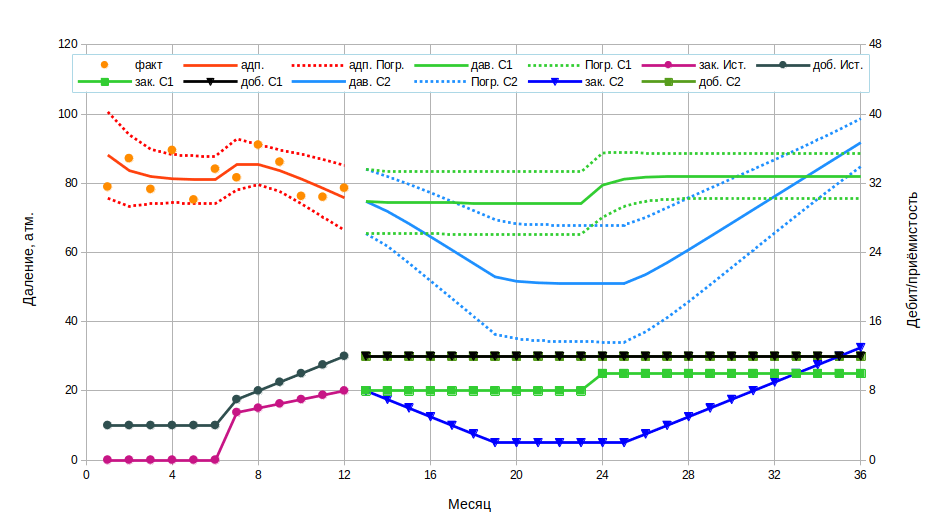
\includegraphics[width=14pc]{1.png}}
		\end{minipage} \hfill
		\begin{minipage}[h]{0.49\linewidth}
			\center{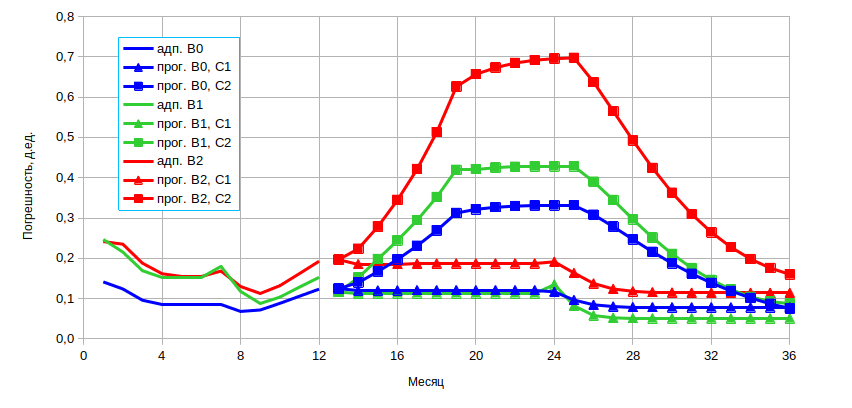
\includegraphics[width=14pc]{2.png}}
		\end{minipage}
		\caption{Схема расположения скважин]}
		\label{fig:map}
	\end{figure}
	
	\section{Пятиточка}
	\begin{figure}
		\center{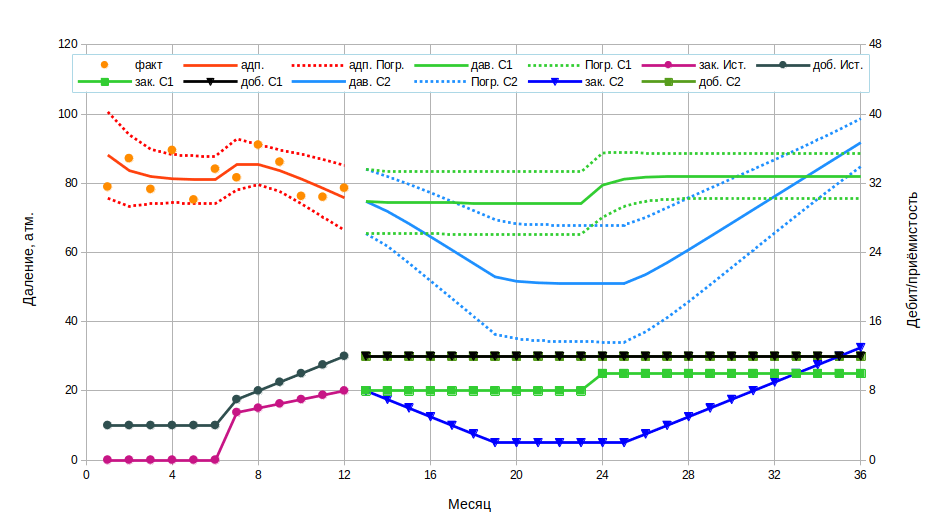
\includegraphics[width=14pc]{1.png}}
		\caption{Значение ЦФ полный перебор]}
		\label{fig:map}
	\end{figure}
	\begin{figure}
		\center{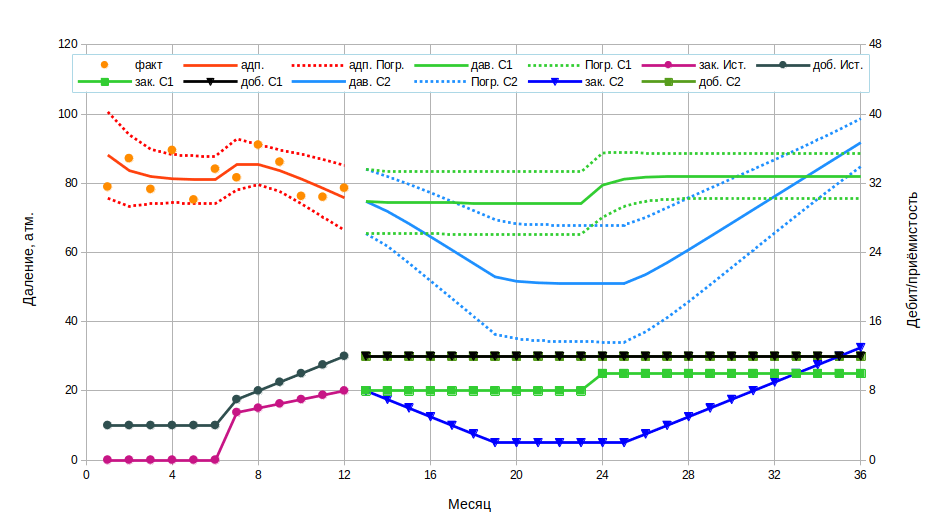
\includegraphics[width=14pc]{1.png}}
		\caption{Наилучшая схема назначения скважин]}
		\label{fig:map}
	\end{figure}
	\begin{figure}
		\center{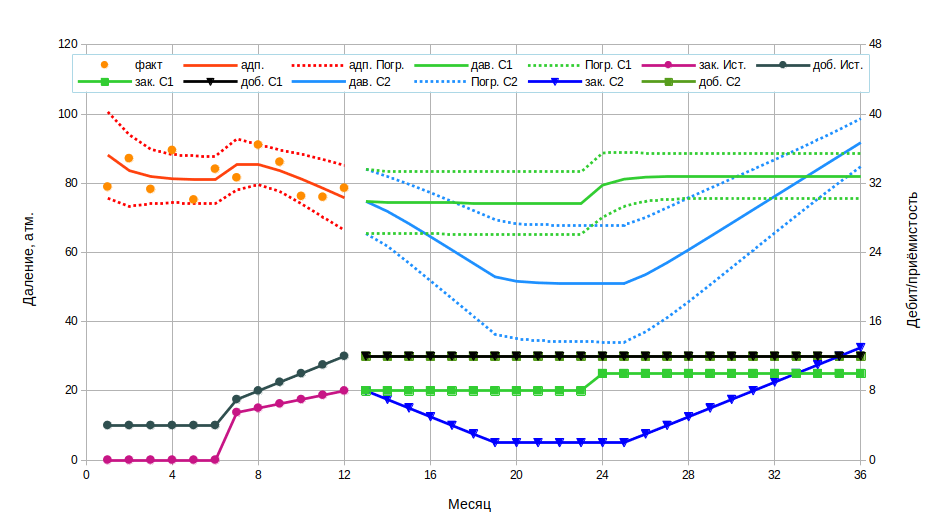
\includegraphics[width=14pc]{1.png}}
		\caption{Схема расположения скважин]}
		\label{fig:map}
	\end{figure}
	
	\section{Девятиточка}
	\begin{figure}
		\center{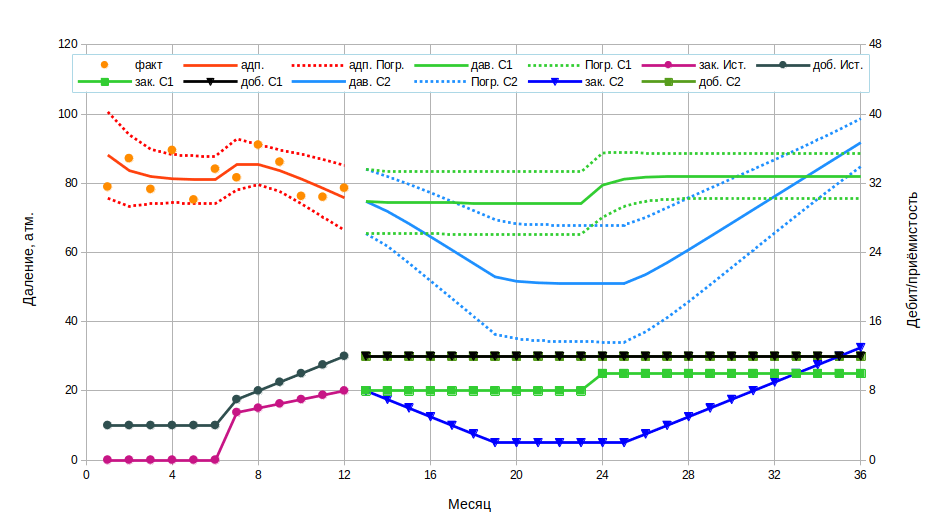
\includegraphics[width=24pc]{1.png}}
		\caption{Значение ЦФ полный перебор]}
		\label{fig:map1}
	\end{figure}
	\begin{figure}
		\center{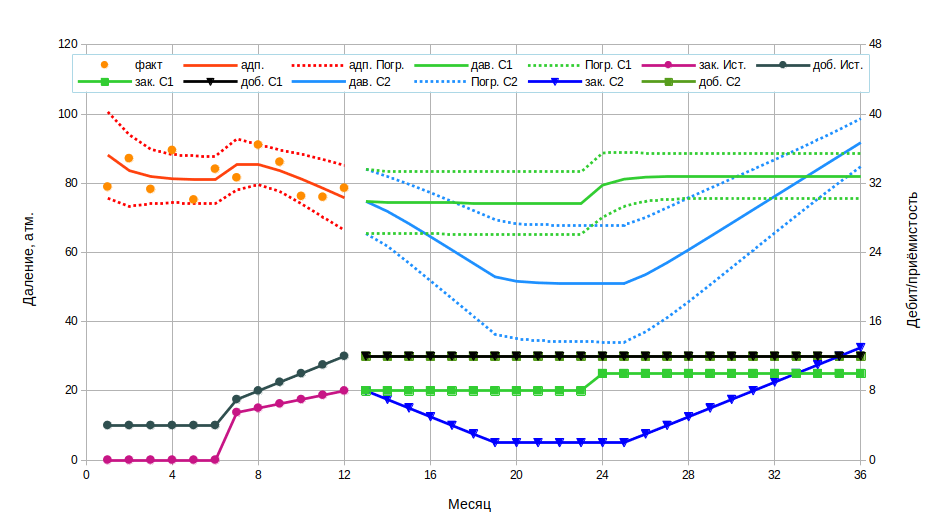
\includegraphics[width=24pc]{1.png}}
		\caption{Наилучшая схема назначения скважин]}
		\label{fig:map2}
	\end{figure}
	\begin{figure}
		\center{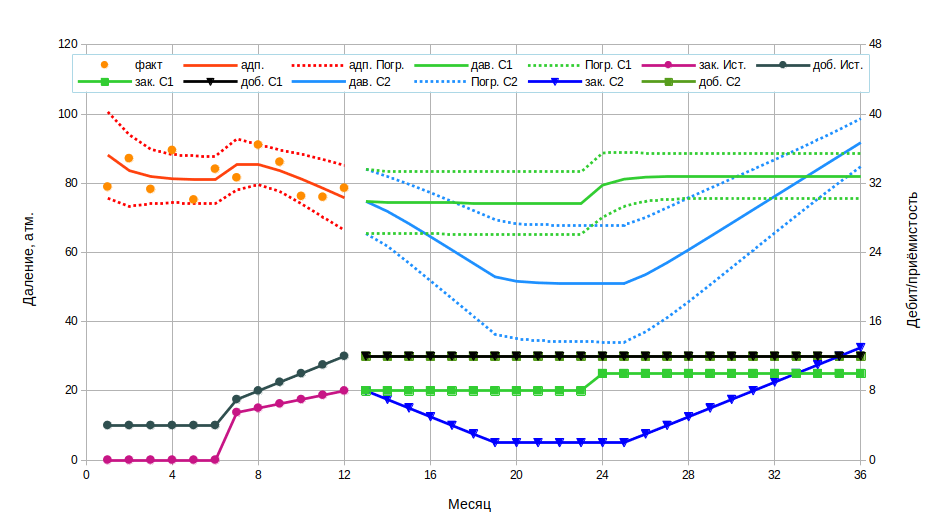
\includegraphics[width=24pc]{1.png}}
		\caption{Схема расположения скважин]}
		\label{fig:map3}
	\end{figure}
	\begin{figure}
		\center{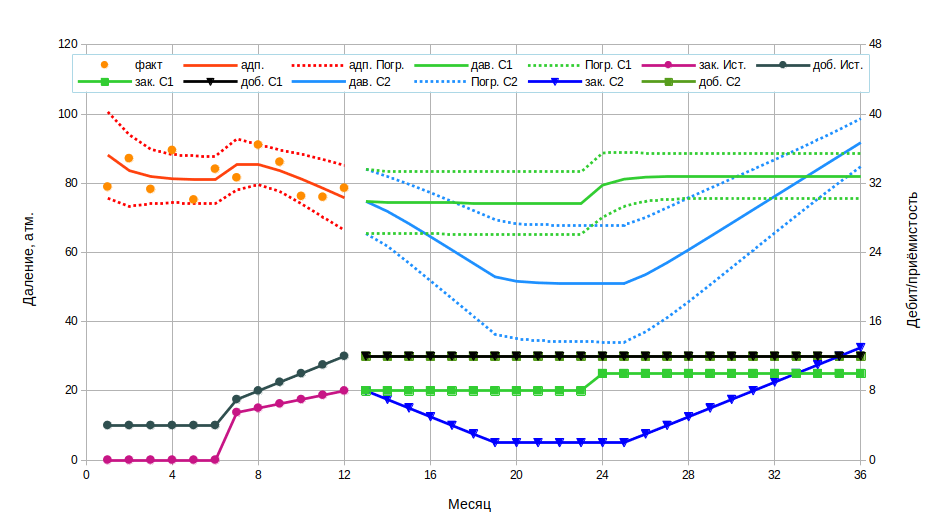
\includegraphics[width=24pc]{1.png}}
		\caption{Схема расположения скважин]}
		\label{fig:map4}
	\end{figure}
	
\end{document}